
\section{Minimize Human Intervention}

\subsection{Ausgangslage}

Für viele Fehler in Systemen sind deren Benutzer verantwortlich, da sie mit falscher Anwendung diese provozieren.
\subsection{Lösungsansatz}

Es gibt drei Kategorien von Fehler in Systemen:
\begin{enumerate}
	\item Hardware
	\item Software
	\item Prozedurale
\end{enumerate}


\subsubsection*{Vergessene Aktionen}

Grundsätzlich verhalten sich Personen schlechter als Computer, wenn sie immer dieselben Schritte (Prozeduren) durchlaufen müssen. Ein Computer haltet sich strikt an die vorgegebene Reihenfolge (ausser Ausnahmen sind explizit zugelassen), eine Person hingegen kann einzelne Schritte überspringen, sei das nun weil sie diesen vergessen oder absichtlich nicht erledigt hat. Läuft ein System fehlerfrei, dann wird diesem System weniger Aufmerksamkeit geschenkt, und dabei können wichtige Aktionen vergessen gehen, falls diese dennoch erwartet werden.
Tritt ein Fehler auf, kann ein Computer viel schneller reagieren als eine Person, die das System bedient.

\subsubsection*{Unerlaubten Aktionen}

Es kann aber auch vorkommen, dass eine Person denkt, dass ein System nicht mehr richtig funktioniert, obwohl dies nicht der Fall ist. Dieser Umstand ist darauf zurückzuführen, dass einer Person nicht genügend Feedback gegeben wird, dass ein System noch am Arbeiten ist. Die einfachste Form hierfür ist eine Progressbar oder die animierten Mauszeiger, welche aus den Betriebssystemen bekannt ist.
Im Allgemeinen gilt: „A quite system is a dead system“
Tritt diese Situation ein, kann es sein, das seine Person Aktionen auslöst, die nicht erwartet werden und die Situation meist verschlechtern. So kann sie einen einwandfrei laufenden Prozess abschalten oder weitere Prozesse starten, die das System noch mehr auslasten.
\subsection{Schlussfolgerung}

Ein System soll so designet werden, dass es selbst Fehler behandeln und automatisch wieder einen normalen Zustand erreicht. Dies führt zu einer schnelleren Fehlerbehandlung, kürzerer Ausfallzeit und es wird vermieden, dass Prozedurale-Fehler während der Behandlung eines Fehlers auftreten können.

\begin{figure}[H]
	\centering
	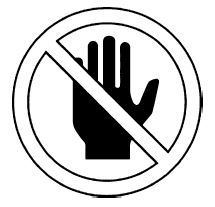
\includegraphics{content/faulttolerance/images/MinimizeHumanIntervention.JPG}
	\caption{MinimizeHumanIntervention}
\end{figure}


Erreicht kann dies wie folgt werden:
\begin{enumerate}
	\item Fehler müssen einem Fault Observer (10) gemeldet werden.
	\item Es dürfen keine internen Meldungen nach aussen gesandt werden.
	\item Die Unit of Mitigation (1) soll Fehler selbst erkennen, behandeln und beheben können, ohne dafür auf Interaktion mit einer Person angewiesen zu sein.
\end{enumerate}

Fehlerbehandlung:
\begin{itemize}
	\item Recovery Blocks (4)
	\item Error Handler (30)
\end{itemize}

Vermeidung von Prozeduralen-Fehlern:
\begin{itemize}
	\item Maximize Human Participation (6)
	\item Maintainance Interfaces (7)
	\item Reintegration (59)
	\item Revise Procedure (63)
\end{itemize}

